% =====================================================================
\chapter{Thiết kế và phân tích kiến trúc}\label{chap:thietke}
% =====================================================================

Chương này đi từ tổng thể đến chi tiết: kiến trúc triển khai và mạng
(\S\ref{sec:trienkhai}), kiến trúc phần mềm máy chủ (\S\ref{sec:phanlop}), mô hình
tác vụ và đồng bộ (\S\ref{sec:tacvu}), các luồng hoạt động (\S\ref{sec:luong}), máy
trạng thái (\S\ref{sec:fsm}), giao thức (\S\ref{sec:giaothuc}), thiết kế chi tiết
từng module (\S\ref{sec:chitiet}), phân tích chất lượng kiến trúc (\S\ref{sec:phantich})
và demo (\S\ref{sec:demo}).

% ---------------------------------------------------------------------
\section{Kiến trúc triển khai và mạng}\label{sec:trienkhai}
\begin{figure}[H]
\centering
\mmd[1][0.6]{deploy}
\caption{Kiến trúc triển khai: máy chủ, hai client và điện thoại cùng là trạm của mạng Wi-Fi chung có Internet; máy chủ ra Internet để hỏi SePay}\label{fig:deploy}
\end{figure}

Hình~\ref{fig:deploy} cho thấy cấu trúc mạng hình sao quanh router (hoặc điểm phát
trên điện thoại) của nhóm: không bo nào phát điểm truy cập, cả ba bo và điện thoại
của người vận hành đều là trạm Wi-Fi. Bảng~\ref{tab:netparams} liệt kê thông số mạng.
Hai client gửi tới địa chỉ \emph{broadcast giới hạn} \code{255.255.255.255} nên không
cần biết dải mạng hay IP máy chủ; người dùng truy cập bằng tên \code{parking.local}
nên cũng không cần biết IP. Router còn cho máy chủ đường ra Internet để kiểm tra
chuyển khoản qua SePay (mục~\ref{sec:vietqr}). Vì tất cả đều là trạm và tự kết nối
lại, thứ tự bật nguồn các bo không còn quan trọng.

\begin{table}[H]
\centering\small
\caption{Thông số mạng}\label{tab:netparams}
\begin{tabularx}{\linewidth}{@{}lX@{}}
\toprule
SSID / mật khẩu & Tên và mật khẩu mạng Wi-Fi chung của nhóm; mặc định \code{ESP32-Parking} / \code{12345678}. Máy chủ: \code{idf.py menuconfig → Parking network and security}; hai client: \file{secrets.h} \\
Điểm truy cập & Router hoặc điểm phát Wi-Fi (điện thoại) của nhóm, có Internet, cấp IP bằng DHCP; phải \emph{tắt} chế độ cô lập thiết bị (AP/client isolation) \\
Máy chủ & Trạm Wi-Fi, IP do DHCP cấp, tên \code{parking.local}, dịch vụ \code{\_http.\_tcp} cổng 80 \\
UDP & Máy chủ nghe cổng 3333; client gửi tới \code{255.255.255.255:3333}; máy chủ trả ACK (unicast) cho sự kiện quẹt thẻ \\
HTTP & Cổng 80: trang web, \code{/api/parking}, \code{/api/barrier}, \code{/api/rfid}, \code{/api/time}, \code{/api/payment/confirm}; lệnh POST cần mã PIN \\
\bottomrule
\end{tabularx}
\end{table}

\begin{lydo}[Tại sao dùng chung một mạng Wi-Fi có Internet và máy chủ dùng mDNS]
Một mạng Wi-Fi chung (router hoặc điểm phát của nhóm) cho máy chủ \textbf{đường ra
Internet} để hỏi SePay xem đã nhận được chuyển khoản chưa — điều không làm được khi
mạng do một bo ESP8266 tự phát. ESP32-C3 chỉ là trạm nên \textbf{không tốn RAM} cho bộ
đệm từng trạm và DHCP server, dành RAM cho màn hình và TLS. Điện thoại của người vận
hành vốn đã ở trong mạng đó nên mở \code{parking.local} ngay mà không phải đổi Wi-Fi.
Đổi lại, bãi \textbf{phụ thuộc vào router} đó; một số router/điểm phát bật chế độ
\emph{cô lập thiết bị} (AP/client isolation) chặn gói broadcast giữa các thiết bị — chế độ
này phải tắt. Mất Internet thì bãi vẫn chạy, chỉ việc xác nhận chuyển khoản chuyển sang
người vận hành. IP máy chủ do DHCP cấp và có thể thay đổi; mDNS giải quyết bằng một
tên cố định \code{parking.local}. Máy chủ còn \emph{chủ động thông báo lại} tên này mỗi
khi nhận địa chỉ mới (sự kiện \code{IP\_EVENT\_STA\_GOT\_IP}), kể cả khi DHCP đổi địa chỉ
mà không mất kết nối, nên các thiết bị khác không bao giờ giữ một IP cũ.
\end{lydo}

\subsection{Giao thức truyền: UDP broadcast}
\begin{table}[H]
\centering\small
\caption{So sánh giao thức truyền dữ liệu cảm biến}\label{tab:proto}
\begin{tabularx}{\linewidth}{@{}lXXX@{}}
\toprule
& \textbf{UDP} & \textbf{HTTP/TCP} & \textbf{MQTT} \\ \midrule
Thiết lập kết nối & Không & Bắt tay 3 bước & Cần broker \\
Overhead/bản tin & 8 byte & Vài trăm byte & 2+ byte trên TCP \\
Bộ nhớ máy chủ & 1 socket, đệm 256\,B & Socket + đệm mỗi kết nối & Thêm broker \\
Khi mất gói & Mất, bản tin sau bù lại & Tự truyền lại & Có QoS \\
\bottomrule
\end{tabularx}
\end{table}

\begin{lydo}
Sensor Client gửi \textbf{toàn bộ trạng thái} (không phải ``sự kiện thay đổi''), và
nhắc lại mỗi giây. Mất một gói chỉ làm trễ tối đa 1\,s, không làm sai trạng thái lâu
dài, nên độ tin cậy của TCP là không cần thiết, trong khi chi phí của nó (bắt tay,
socket, bộ đệm) đáng kể trên vi điều khiển. Gửi broadcast giới hạn
\code{255.255.255.255} giúp client không cần biết dải mạng của router hay IP máy chủ
và cho phép máy tính trong mạng ``nghe'' để gỡ lỗi. JSON được chọn vì đọc
được trong log và dễ sinh từ \code{snprintf}/Python; bản tin dài 70–130 byte, nằm
gọn trong một gói UDP.

Sự kiện quẹt thẻ thì khác: nó \emph{không} được nhắc lại, mất gói là mất lượt quẹt.
Thay vì chuyển sang TCP, nhóm thêm đúng phần độ tin cậy cần thiết: máy chủ trả
\code{ACK} cho từng sự kiện, RFID Client gửi lại sau 300\,ms nếu chưa nhận được, và
số thứ tự giúp máy chủ nhận ra bản gửi lại để không mở cổng hai lần.
\end{lydo}

% ---------------------------------------------------------------------
\section{Kiến trúc phần mềm máy chủ}\label{sec:phanlop}
Firmware máy chủ được tổ chức theo \textbf{kiến trúc phân lớp} (Hình~\ref{fig:layers}):
mỗi lớp chỉ gọi lớp dưới nó. Lớp \emph{nghiệp vụ} (\file{parking/}) không phụ thuộc
phần cứng nên chạy được cả trên máy tính để kiểm thử.

\begin{figure}[H]
\centering
\begin{tikzpicture}[
  lay/.style={draw,thick,rounded corners=2pt,minimum height=1.05cm,align=center,font=\small},
  mod/.style={draw,rounded corners=2pt,fill=white,font=\scriptsize,align=center,minimum height=0.62cm,inner sep=2pt}]
\def\W{14.6}
\node[lay,fill=boxE,minimum width=\W cm] (app) at (0,4.2) {};
\node[anchor=west,font=\small\bfseries] at (-7.2,4.2) {Ứng dụng};
\node[mod] at (0.9,4.2) {\texttt{main.c}: khởi động theo thứ tự, fail-fast};
\node[lay,fill=boxA,minimum width=\W cm,minimum height=1.35cm] (svc) at (0,2.75) {};
\node[anchor=west,font=\small\bfseries,align=left] at (-7.2,2.75) {Dịch vụ};
\node[mod,minimum width=2.1cm] at (-3.4,2.75) {\texttt{udp\_server}\\điều phối bản tin};
\node[mod,minimum width=2.1cm] at (-1.05,2.75) {\texttt{http\_server}\\web + API};
\node[mod,minimum width=2.1cm] at (1.3,2.75) {\texttt{lcd\_display}\\giao diện TFT};
\node[mod,minimum width=1.6cm] at (3.35,2.75) {\texttt{servo}\\thanh chắn};
\node[mod,minimum width=1.4cm] at (5.05,2.75) {\texttt{buzzer}};
\node[mod,minimum width=1.4cm] at (6.45,2.75) {\texttt{network}\\Wi-Fi, mDNS};
\node[lay,fill=boxB,minimum width=\W cm] (dom) at (0,1.2) {};
\node[anchor=west,font=\small\bfseries,align=left] at (-7.2,1.2) {Nghiệp vụ};
\node[mod] at (-3.4,1.2) {\texttt{parking\_state}\\trạng thái, đồng hồ};
\node[mod] at (-0.2,1.2) {\texttt{json\_scan}, \texttt{parking\_update}\\kiểm tra bản tin};
\node[mod] at (3.6,1.2) {\texttt{rfid\_session}\\phiên, phí, nhật ký, lưu/khôi phục};
\node[lay,fill=boxC,minimum width=\W cm] (drv) at (0,-0.3) {};
\node[anchor=west,font=\small\bfseries,align=left] at (-7.2,-0.3) {ESP-IDF};
\node[mod] at (-3.5,-0.3) {\code{esp\_lcd} · SPI DMA};
\node[mod] at (-1.0,-0.3) {LEDC · GPIO};
\node[mod] at (1.2,-0.3) {\code{esp\_timer}};
\node[mod] at (3.2,-0.3) {lwIP · HTTPD};
\node[mod] at (5.6,-0.3) {Wi-Fi · mDNS · NVS};
\node[lay,fill=boxD,minimum width=\W cm] (os) at (0,-1.6) {};
\node[anchor=west,font=\small\bfseries,align=left] at (-7.2,-1.6) {RTOS};
\node[mod] at (0.9,-1.6) {FreeRTOS: tác vụ, mutex, critical section, thông báo tác vụ};
\node[lay,fill=gray!15,minimum width=\W cm,minimum height=0.8cm] (hw) at (0,-2.8) {\textbf{Phần cứng}: ESP32-C3 — SPI2, LEDC, GPIO, Wi-Fi};
\end{tikzpicture}
\caption{Kiến trúc phân lớp của firmware máy chủ}\label{fig:layers}
\end{figure}

\subsection{Phụ thuộc giữa các module}
Hình~\ref{fig:deps} là đồ thị phụ thuộc: mũi tên từ A đến B nghĩa là A gọi B. Mọi
mũi tên đều đi xuống lớp thấp hơn, hoặc từ \file{udp\_server} sang các thiết bị cùng
lớp dịch vụ, nên không có vòng phụ thuộc.

\begin{figure}[H]
\centering
\mmd[0.95][0.6]{deps}
\caption{Đồ thị phụ thuộc giữa các module (tím: ứng dụng, xanh dương: dịch vụ, xanh lá: nghiệp vụ, cam: dữ liệu)}\label{fig:deps}
\end{figure}

\begin{lydo}[Tại sao phân lớp như vậy]
(1) \emph{Kiểm thử được}: \file{parking\_state}, \file{json\_scan}, \file{parking\_update},
\file{rfid\_session}, \file{payment} chỉ cần hai macro critical section và hàm đọc đồng hồ — thay bằng
hai tệp header giả là chạy được trên máy tính. (2) \emph{Thay đổi cục bộ}: đổi màn hình
khác chỉ sửa \file{lcd\_display}; đổi giao thức mạng chỉ sửa \file{udp\_server}.
Việc ghi flash nằm riêng trong \file{parking\_persist}: \file{rfid\_session} chỉ đưa ra
một ``ảnh chụp'' trạng thái (\code{rfid\_store\_t}) nên vẫn kiểm thử được trên máy tính.
(3) \emph{Không vòng phụ thuộc} (Hình~\ref{fig:deps}): \file{udp\_server} là nơi
``điều phối'' bản tin — nhận bản tin, gọi nghiệp vụ, rồi ra lệnh cho servo, còi và đánh
thức màn hình; \file{sepay\_client} làm đúng việc đó cho kết quả thanh toán. Phần đọc
JSON của SePay và dựng chuỗi QR nằm trong \file{payment}, không gọi mạng, nên kiểm thử
được trên máy tính.
\end{lydo}

% ---------------------------------------------------------------------
\section{Mô hình tác vụ và đồng bộ}\label{sec:tacvu}
\begin{table}[H]
\centering\small
\caption{Các tác vụ đang chạy trên máy chủ}\label{tab:tasks}
\begin{tabularx}{\linewidth}{@{}lccp{3.0cm}X@{}}
\toprule
\textbf{Tác vụ} & \textbf{Ưu tiên} & \textbf{Stack} & \textbf{Đánh thức bởi} & \textbf{Nhiệm vụ} \\ \midrule
\code{udp\_server} & 5 & 4096 B & gói UDP đến & Kiểm tra bản tin, cập nhật trạng thái, ra lệnh servo/còi/màn hình \\
\code{httpd} & 5 & 4096 B & yêu cầu HTTP & Trang web, API \\
\code{esp\_timer} (hệ thống) & cao & 3584 B & hẹn giờ & Gọi hàm đóng thanh chắn khi hết 3\,s \\
\code{lcd\_display} & 4 & 4096 B & thông báo tác vụ / 1\,s / 120\,ms & Vẽ lại màn hình khi dữ liệu đổi \\
\code{lcd\_animation} & 3 & 3072 B & mỗi khung (100\,ms) & Ảnh động trang trí \\
\code{sepay} & 3 & 8192 B & mỗi 1\,s; mỗi 3\,s khi có xe đang thanh toán & Hỏi API SePay qua HTTPS, hoàn tất thanh toán và mở cổng ra; chỉ tạo khi có token SePay \\
\code{mdns} & 1 & 4096 B & gói mDNS & Trả lời \code{parking.local} \\
\bottomrule
\end{tabularx}
\end{table}

\begin{figure}[H]
\centering
\mmd[0.95][0.6]{tasks}
\caption{Tác vụ (xanh dương, kèm mức ưu tiên), tài nguyên dùng chung (xanh lá) và cơ chế bảo vệ; nét đứt đỏ: đánh thức tác vụ}\label{fig:tasks}
\end{figure}

Hệ thống dùng \textbf{ba cơ chế đồng bộ} cho ba loại tình huống khác nhau:
\begin{itemize}
\item \textbf{Critical section} (\code{portENTER\_CRITICAL}) cho \file{parking\_state} và
  \file{rfid\_session}: vùng bảo vệ chỉ là vài lệnh sao chép cấu trúc nhỏ (vài micro
  giây). Cách này rẻ hơn mutex; người đọc luôn nhận một bản sao nhất quán.
\item \textbf{Mutex} cho servo và panel LCD: vùng bảo vệ dài hơn (gửi dữ liệu SPI,
  ghi thanh ghi LEDC) và có thể chờ; mutex không tắt ngắt, cho phép tác vụ khác chạy
  và có cơ chế kế thừa ưu tiên để chống đảo ưu tiên.
\item \textbf{Thông báo tác vụ} (\code{xTaskNotifyGive}/\code{ulTaskNotifyTake}) để
  \file{udp\_server} đánh thức \file{lcd\_display} ngay khi có dữ liệu mới — nhẹ hơn
  semaphore (không cấp phát đối tượng) và thay cho việc hỏi vòng 500\,ms trước đây.
\end{itemize}

\begin{lydo}[Tại sao đặt ưu tiên như vậy]
Ưu tiên phản ánh mức độ quan trọng với người dùng: nhận bản tin và điều khiển thanh
chắn (5) liên quan trực tiếp đến xe đang chờ ở cổng; màn hình thông tin (4) quan
trọng hơn ảnh động trang trí (3); tác vụ SePay (3) chờ mạng Internet hàng trăm mili
giây mỗi lần nên không được chen trước việc điều khiển cổng; mDNS (1) chỉ trả lời truy vấn tên, chậm vài mili
giây không ảnh hưởng. Khi CPU bận, ảnh động chậm đi chứ thông tin không bị trễ.
\end{lydo}

% ---------------------------------------------------------------------
\section{Luồng hoạt động}\label{sec:luong}
\subsection{Khởi động máy chủ}
\begin{figure}[H]
\centering
\mmd[1][0.72]{boot}
\caption{Trình tự khởi động máy chủ (\file{main.c})}\label{fig:boot}
\end{figure}

\begin{lydo}[Tại sao thứ tự khởi động như vậy]
\textbf{NVS trước tiên} vì Wi-Fi đọc dữ liệu hiệu chuẩn từ NVS. \textbf{Màn hình
trước Wi-Fi}: framebuffer cần một khối bộ nhớ \emph{liền mạch} 115\,KB có khả năng
DMA; Wi-Fi cấp phát nhiều khối nhỏ làm phân mảnh heap, nên phải lấy khối lớn trước.
\textbf{Còi và servo trước mạng}: đưa còi về im lặng và thanh chắn về vị trí đóng
trước khi có bất kỳ lệnh nào từ mạng. \textbf{Mạng sau cùng}: chỉ nhận lệnh khi mọi
thiết bị đã sẵn sàng. \code{ESP\_ERROR\_CHECK} áp dụng nguyên tắc \emph{fail-fast}:
lỗi khởi tạo dẫn tới khởi động lại thay vì chạy ở trạng thái nửa vời.
\end{lydo}

\subsection{Xử lý bản tin UDP trên máy chủ}
\begin{figure}[H]
\centering
\mmd[1][0.6]{udpflow}
\caption{Lưu đồ điều phối bản tin trong tác vụ \code{udp\_server}}\label{fig:udpflow}
\end{figure}
Nếu socket lỗi, tác vụ đóng socket, chờ 1\,s rồi tạo lại — tự phục hồi mà không cần
khởi động lại máy chủ. Khi không có gói, tác vụ ngủ trong \code{recvfrom()} và
\textbf{không tốn CPU}.

\subsection{Vòng lặp của hai client}
\begin{figure}[H]
\centering
\mmd[1][0.62]{clientloops}
\caption{Vòng lặp không chặn của Sensor Client và RFID Client}\label{fig:clientloops}
\end{figure}

\subsection{Xe vào và ra bằng thẻ RFID}
\begin{figure}[H]
\centering
\mmd[1][0.62]{seq_rfid}
\caption{Biểu đồ tuần tự gửi xe (trên) và lấy xe (dưới)}\label{fig:seq-rfid}
\end{figure}

\subsection{Phát hiện cháy}
\begin{figure}[H]
\centering
\mmd[1][0.6]{seq_fire}
\caption{Biểu đồ tuần tự cảnh báo cháy}\label{fig:seq-fire}
\end{figure}

\subsection{Trang web giám sát}
Trình duyệt tải trang một lần, sau đó gọi \code{GET /api/parking} mỗi 1\,s,
\code{GET /api/rfid} mỗi 2\,s và \code{GET /api/barrier} khi mở trang. Lệnh điều
khiển dùng \code{POST}; các nút bị khóa đến khi có phản hồi để tránh gửi trùng.

% ---------------------------------------------------------------------
\section{Máy trạng thái}\label{sec:fsm}
\begin{figure}[H]
\centering
\mmd[1][0.6]{fsm_card}
\caption{Máy trạng thái của một thẻ RFID}\label{fig:fsm-card}
\end{figure}

\begin{figure}[H]
\centering
\mmd[1][0.6]{fsm_gate}
\caption{Máy trạng thái của một thanh chắn}\label{fig:fsm-gate}
\end{figure}

\begin{figure}[H]
\centering
\mmd[1][0.6]{fsm_footer}
\caption{Trạng thái vùng chân màn hình (footer) TFT; khi có cháy, toàn màn hình chuyển sang màn hình cảnh báo}\label{fig:fsm-footer}
\end{figure}

% ---------------------------------------------------------------------
\section{Giao thức và giao diện lập trình}\label{sec:giaothuc}
\begin{lstlisting}[language=json,caption={Bản tin \code{parking\_update} (Sensor Client → máy chủ)}]
{"type":"parking_update","slots":[1,0,0,1,0],"water_mm":0.2,"fire":false}
\end{lstlisting}
\begin{lstlisting}[language=json,caption={Bản tin \code{rfid\_event} (RFID Client → máy chủ)}]
{"type":"rfid_event","card_id":"A1B2C3D4","gate":"in","temperature_c":28.0}
\end{lstlisting}
\begin{lstlisting}[language=json,caption={Bản tin \code{climate} (RFID Client → máy chủ, mỗi 5\,s)}]
{"type":"climate","temperature_c":28.0}
\end{lstlisting}

\paragraph{Xác nhận sự kiện quẹt thẻ.} Bản tin \code{rfid\_event} có thêm trường \code{seq}
(số nguyên 32 bit, khác 0) do RFID Client đặt; máy chủ trả lời bằng một gói JSON cùng
\code{seq}:
\begin{lstlisting}[language=json,caption={Sự kiện quẹt thẻ và gói xác nhận}]
{"type":"rfid_event","card_id":"A1B2C3D4","gate":"in","temperature_c":28.0,"seq":305441741}
{"type":"rfid_ack","seq":305441741}
\end{lstlisting}
\begin{itemize}[nosep]
  \item RFID Client gửi lại đúng gói đó mỗi 300\,ms (tối đa 6 lần) cho tới khi nhận được ACK.
  \item Máy chủ nhớ 16 giá trị \code{seq} gần nhất: gặp lại một \code{seq} đã xử lý là bản
        gửi lại, chỉ trả ACK chứ không mở cổng lần hai.
  \item \code{seq} bắt đầu từ một số ngẫu nhiên (bộ sinh số ngẫu nhiên phần cứng của
        ESP8266) mỗi lần khởi động rồi tăng dần, nên gần như không trùng với số máy chủ
        vừa thấy; client không cần lưu gì vào flash.
\end{itemize}

\begin{lydo}[Tại sao không ký (xác thực) gói UDP]
Ba bo nằm trong mạng Wi-Fi riêng của nhóm, được bảo vệ bằng WPA2; chỉ thiết bị
biết mật khẩu Wi-Fi mới gửi được gói tin. Ở quy mô mô hình, nhóm ưu tiên giao thức đơn
giản, đọc được trực tiếp trong log và dễ giả lập bằng script. Các thao tác nhạy cảm từ
trình duyệt (mở cổng, đặt giờ) vẫn cần mã PIN. Ký gói bằng mã xác thực (HMAC) được để
lại cho hướng phát triển.
\end{lydo}

\begin{table}[H]
\centering\small
\caption{Đặc tả trường dữ liệu và ràng buộc kiểm tra trên máy chủ}\label{tab:fields}
\begin{tabularx}{\linewidth}{@{}llX@{}}
\toprule
\textbf{Trường} & \textbf{Kiểu} & \textbf{Ràng buộc} \\ \midrule
\code{type} & chuỗi & \code{"parking\_update"}, \code{"rfid\_event"} hoặc \code{"climate"} \\
\code{seq} & số nguyên & Chỉ trong \code{rfid\_event}; $1 \le x \le 2^{32}-1$, không dấu, không phần thập phân \\
\code{slots} & mảng & Đúng 5 phần tử, mỗi phần tử 0 (trống) hoặc 1 (có xe) \\
\code{water\_mm} & số & $0 \le x \le 10\,000$ \\
\code{fire} & boolean & Tùy chọn (client cũ có thể không gửi); không chấp nhận 0/1 \\
\code{card\_id} & chuỗi & 1–31 ký tự \code{[A-Za-z0-9\_-]}, chuẩn hóa thành chữ hoa \\
\code{gate} & chuỗi & \code{"in"} hoặc \code{"out"} (không phân biệt hoa thường) \\
\code{temperature\_c} & số & $-40 \le x \le 125$ \\
Chung & — & Khóa lạ, khóa lặp, dữ liệu thừa sau \code{\}}, chuỗi có ký tự thoát đều bị từ chối \\
\bottomrule
\end{tabularx}
\end{table}

\begin{table}[H]
\centering\small
\caption[API HTTP của máy chủ (13 route)]{API HTTP của máy chủ (13 route); mọi lệnh POST cần header \code{X-Parking-Key} đúng mã PIN, sai thì trả 401}\label{tab:api}
\begin{tabularx}{\linewidth}{@{}lp{4.4cm}X@{}}
\toprule
\textbf{PT} & \textbf{Đường dẫn} & \textbf{Kết quả} \\ \midrule
GET & \code{/}, \code{/style.css} & Trang web nhúng trong firmware \\
GET & \code{/api/parking} & \code{received}, \code{online}, \code{slots}, \code{free}, \code{total}, \code{temperature\_c}, \code{water\_mm}, \code{fire}, \code{flood} \\
GET & \code{/api/barrier} & \code{\{"in\_open":bool,"out\_open":bool\}} \\
GET & \code{/api/rfid} & \code{now\_s}, \code{fee\_per\_hour}, \code{today}/\code{week} (doanh thu, lượt vào, lượt ra), \code{parked[]} (thẻ, giờ vào, phí tạm tính), \code{payment} (lượt thanh toán đang chờ: \code{\{"card","fee","code","expired"\}} hoặc \code{null}), \code{log[]} (10 sự kiện mới nhất) \\
POST & \code{/api/barrier/}\allowbreak\code{<cổng>/<lệnh>} & Cổng \code{in}, \code{out}, \code{all}; lệnh \code{open}, \code{close}. Lỗi 500 nếu bị từ chối (ví dụ đóng khi có cháy) \\
POST & \code{/api/time} & Thân là giờ Unix (giây) từ trình duyệt; máy chủ đặt đồng hồ bãi và lưu NVS \\
POST & \code{/api/payment/confirm} & Thân là mã thẻ; người vận hành xác nhận đã nhận tiền (chuyển khoản hoặc tiền mặt): xe ra như bình thường. Dùng được cả cho xe chưa quẹt ra (thu phí đến hiện tại) \\
\bottomrule
\end{tabularx}
\end{table}

% ---------------------------------------------------------------------
\section{Thiết kế chi tiết từng thành phần}\label{sec:chitiet}

\subsection{Thanh chắn: PWM phần cứng và hẹn giờ một lần}
Servo SG90 nhận xung chu kỳ 20\,ms; độ rộng xung quyết định góc (Hình~\ref{fig:pwm}).
\begin{figure}[H]
\centering
\begin{tikzpicture}[x=0.55cm,y=0.7cm,font=\scriptsize]
\draw[-{Stealth}] (0,0) -- (23,0) node[right]{$t$ (ms)};
\draw[-{Stealth}] (0,0) -- (0,1.8) node[left]{PWM};
\draw[thick,accent] (0,0) -- (0,1.2) -- (1.45,1.2) -- (1.45,0) -- (20,0) -- (20,1.2) -- (21.45,1.2) -- (21.45,0) -- (22.5,0);
\draw[{Stealth}-{Stealth}] (0,-0.5) -- node[below]{chu kỳ $T = 20$\,ms (50\,Hz)} (20,-0.5);
\draw[{Stealth}-{Stealth}] (0,1.5) -- node[above]{$p$} (1.45,1.5);
\node[align=left,anchor=west] at (3,1.0) {$p = 500$\,µs $\to 0°$\quad $p = 1450$\,µs $\to 90°$\quad $p = 2400$\,µs $\to 180°$};
\end{tikzpicture}
\caption{Dạng xung điều khiển servo SG90}\label{fig:pwm}
\end{figure}
\begin{equation}
  p(\theta) = 500 + \frac{1900\,\theta}{180}\ \text{µs}, \qquad
  D = \left\lfloor \frac{p \cdot (2^{14}-1)}{20\,000} \right\rfloor
\end{equation}
Với $\theta=90°$: $p=1450$\,µs, $D=1187$; với $\theta=0°$: $p=500$\,µs, $D=409$.

\begin{lydo}[Tại sao 50\,Hz, 14 bit, LEDC]
\textbf{50\,Hz} là tần số chuẩn của servo RC analog. \textbf{14 bit} là độ phân giải
lớn nhất của LEDC trên ESP32-C3: mỗi bước $20\,000/16\,384 \approx 1{,}22$\,µs $\approx 0{,}12°$,
mịn hơn nhiều vùng chết $\approx$1° của SG90 nên servo không rung. \textbf{LEDC} là PWM
phần cứng: xung phát liên tục mà CPU không can thiệp, servo giữ góc ổn định dù
Wi-Fi hay màn hình đang bận. Dải 500–2400\,µs là giá trị đo thực tế của SG90 (danh
nghĩa 1000–2000\,µs không đủ 180°).
\end{lydo}

\begin{lydo}[Tại sao dùng hẹn giờ một lần (\code{esp\_timer}) thay vì tác vụ hỏi vòng]
Phiên bản đầu dùng một tác vụ thức dậy 20 lần/giây để kiểm tra hạn đóng. Phiên bản
hiện tại tạo một \code{esp\_timer} một lần cho mỗi cổng: hàm đóng được gọi \emph{đúng}
lúc hết 3\,s (sai số micro giây thay vì 50\,ms), CPU không bị đánh thức vô ích và tiết
kiệm 3\,KB stack. Vì một lệnh khác có thể ``đua'' với hàm đóng, hàm đóng kiểm tra lại
hạn đóng dưới mutex; lệnh tay từ web đặt hạn về 0 và dừng hẹn giờ — \textbf{lệnh của
người vận hành luôn thắng}.
\end{lydo}

Hai cổng được mô tả bằng cùng một cấu trúc (kênh LEDC, chân, hướng lắp, trạng thái,
hạn đóng, hẹn giờ) nên một hàm xử lý cho cả hai. Thanh chắn ra lắp đối xứng nên góc
mở/đóng đảo ngược (0° mở, 90° đóng) — chỉ khai báo ở một hàm. Cả hai cổng \textbf{luôn
khởi động ở vị trí đóng}, nên trạng thái không cần lưu vào flash; phiên bản trước ghi
NVS mỗi lần thanh chắn chuyển động đã được bỏ (chậm và làm mòn flash vô ích).

\subsection{Màn hình: SPI DMA, vẽ theo sự kiện, ảnh động tiền xử lý}
\begin{lydo}[Tại sao SPI 40\,MHz và DMA]
Một khung hình đầy đủ là $240\times240\times16 = 921\,600$ bit; ở 40\,MHz mất
$\approx$ 23\,ms, tối đa $\approx$ 43 khung/giây — dư cho giao diện tĩnh và màn hình cháy
8 khung/giây. 40\,MHz bằng đúng $80\,\text{MHz}/2$ (không sai số chia tần) và dưới giới
hạn ghi $\approx$ 62\,MHz của ST7789, chừa biên an toàn cho dây cắm. DMA cho phép CPU
làm việc khác trong lúc ảnh được đẩy ra.
\end{lydo}

\begin{itemize}
\item \textbf{Framebuffer RGB565} 115\,200 byte: toàn bộ giao diện được vẽ vào RAM rồi gửi
  một lần. Màu được lưu sẵn theo thứ tự byte của ST7789 (byte cao trước) vì
  ESP32-C3 là little-endian.
\item \textbf{Hàm tô hình chữ nhật} cắt biên một lần và tô từng dòng liên tục thay vì
  kiểm tra biên và đảo byte cho từng điểm ảnh.
\item \textbf{Font 5$\times$7 tự định nghĩa} cho A–Z, 0–9 (180 byte) — không cần thư viện
  đồ họa lớn như LVGL cho một giao diện cố định.
\item \textbf{Vẽ theo sự kiện}: \file{udp\_server} đánh thức tác vụ màn hình bằng thông
  báo tác vụ ngay khi có dữ liệu; nếu không có gì, tác vụ chỉ thức mỗi 1\,s (để hết hạn
  hóa đơn/thông báo) hoặc 120\,ms khi có cháy (để lửa nhấp nháy). Màn hình chỉ vẽ lại
  khi nội dung thực sự thay đổi.
\end{itemize}

\begin{table}[H]
\centering\small
\caption{Dữ liệu ảnh động sau tiền xử lý và nén LZSS}\label{tab:lzss}
\begin{tabular}{@{}lrrrr@{}}
\toprule
\textbf{Ảnh} & \textbf{Kích thước} & \textbf{Số khung} & \textbf{Dữ liệu thô} & \textbf{Sau nén} \\ \midrule
Kaoruko & 96$\times$96 & 10 & 184\,320 B & 70\,564 B (2,6$\times$) \\
Claude & 68$\times$46 & 18 & 112\,608 B & 16\,204 B (6,9$\times$) \\
\bottomrule
\end{tabular}
\end{table}
\noindent Hai bộ đệm DMA $96\times96$ của ảnh Kaoruko (36\,KB) chính là phần heap mà bắt tay HTTPS
với SePay cần. Vì ảnh động vốn dừng khi đang hiện mã QR, tác vụ \code{lcd\_animation} trả hai bộ đệm
này lại trong lúc có xe đang thanh toán và cấp phát lại sau đó; nếu lúc ấy heap chưa đủ thì chỉ bỏ
qua khung hình. Có thể tắt hẳn ảnh bằng \code{PARKING\_LCD\_KAORUKO} trong menuconfig (góc màn hình
hiện ô chữ ``P'').

\begin{lydo}[Tại sao tiền xử lý ảnh trên máy tính]
Ảnh gốc có nền trắng cần xóa và điểm ảnh cần đảo byte. Phiên bản trước làm việc
này trên chip cho \emph{mọi khung hình}, 10 lần/giây: thuật toán loang tìm nền trắng
nối với viền (cần thêm 1,2\,KB RAM) rồi đảo byte 9\,216 điểm. Vì ảnh không bao giờ
đổi, nhóm làm một lần trên máy tính và lưu kết quả đã xử lý: firmware chỉ còn giải
nén. Kết quả được kiểm chứng giống từng điểm ảnh với cách cũ trên cả 28 khung, dữ
liệu còn nhỏ hơn (86\,768 so với 87\,977 byte). LZSS có bộ giải nén $\approx$ 40 dòng,
không cần bộ nhớ phụ và kiểm tra biên đầy đủ nên dữ liệu hỏng không gây ghi tràn.
\end{lydo}

\textbf{Hai bộ đệm DMA} (2 $\times$ 18\,432 byte) được dùng luân phiên cho ảnh động:
lệnh vẽ chỉ \emph{xếp hàng} giao dịch DMA rồi trả về, nên giải nén khung kế tiếp vào
cùng bộ đệm khi DMA chưa đọc xong sẽ làm hình bị xé. Hai tác vụ cùng vẽ lên một
panel nên dùng chung một mutex.

\subsection{Bộ kiểm tra bản tin JSON}
\begin{lydo}[Tại sao tự viết thay vì dùng thư viện cJSON]
Gói UDP là \emph{ranh giới tin cậy}: bất kỳ thiết bị nào trong mạng đều gửi được.
cJSON cấp phát heap cho từng nút (phân mảnh heap khi chạy lâu) và chấp nhận mọi JSON
hợp lệ. Bộ đọc tự viết (\file{json\_scan.c}, 81 dòng, dùng chung cho cả hai loại bản
tin) \textbf{không cấp phát động}, chỉ chấp nhận đúng lược đồ (Bảng~\ref{tab:fields})
và có \textbf{vòng lặp giới hạn} (tối đa 4 khóa) nên thời gian xử lý bị chặn trên.
Bộ đệm nhận 256 byte, đọc tối đa 255 byte và luôn kết thúc bằng \code{'\textbackslash0'}.
\end{lydo}

\subsection{Phiên gửi xe, phí, thông báo và nhật ký}
\begin{itemize}
\item \textbf{Phiên}: mảng tĩnh 5 phần tử — bằng số chỗ đỗ, vì không thể có nhiều xe hơn số chỗ.
  Thời điểm vào lấy từ \code{esp\_timer\_get\_time()} (64 bit, micro giây, không tràn trong
  hơn 290\,000 năm).
\item \textbf{Phí}: $h=\max(1,\lceil t/3600\rceil)$, phí $=5000\,h$ VNĐ, tính bằng số
  nguyên \code{(t + 3599) / 3600}, bão hòa ở \code{UINT32\_MAX} nếu tràn.
\item \textbf{Thông báo từ chối} (sai cổng, bãi đầy): giữ 5\,s; lần quẹt hợp lệ tiếp
  theo xóa thông báo ngay.
\item \textbf{Nhật ký}: bộ đệm vòng 10 sự kiện ($\approx$ 520 byte), đọc ra theo thứ tự mới
  nhất trước; không dùng heap.
\end{itemize}

\begin{lydo}[Tại sao chọn các thông số này]
\textbf{5.000\,VNĐ/giờ, làm tròn lên, tối thiểu 1 giờ} là cách tính phổ biến của bãi
xe, dễ giải thích. \textbf{Hóa đơn 60\,s} đủ để tài xế đọc và trả tiền; \textbf{thông
báo 5\,s} đủ đọc mà không che hóa đơn quá lâu. \textbf{Thanh chắn mở 3\,s} đủ cho xe mô
hình đi qua nhưng không đủ để xe sau ``đi ké''. \textbf{Nhật ký 10 sự kiện} vừa một màn
hình điện thoại và tốn dưới 1\,KB RAM.
\end{lydo}

\subsection{Thanh toán VietQR qua SePay}\label{sec:vietqr}
Khi thanh toán QR được bật, quẹt thẻ ở cổng ra \emph{không} mở cổng ngay: máy chủ chốt
phí tại thời điểm quẹt, tạo một \textbf{mã thanh toán} và vẽ mã VietQR lên TFT. Mọi ứng
dụng ngân hàng Việt Nam quét được mã này, số tiền và nội dung chuyển khoản đã điền sẵn.
Thanh chắn ra chỉ mở khi máy chủ thấy giao dịch khớp (qua SePay) hoặc người vận hành bấm
\code{Confirm paid} trên trang web (Hình~\ref{fig:seq-pay}).

\paragraph{Chuỗi VietQR.} Hàm \code{vietqr\_payload()} (\file{parking/payment.c}) dựng
chuỗi theo chuẩn VietQR của NAPAS, vốn là định dạng EMVCo: mỗi trường gồm mã 2 chữ số,
độ dài 2 chữ số và giá trị; trường 38 và 62 chứa các trường con theo cùng cách
(Bảng~\ref{tab:vietqr}).
\begin{table}[H]
\centering\small
\caption{Cấu trúc chuỗi VietQR do máy chủ sinh}\label{tab:vietqr}
\begin{tabularx}{\linewidth}{@{}llX@{}}
\toprule
\textbf{Mã} & \textbf{Trường} & \textbf{Giá trị} \\ \midrule
00 & Phiên bản định dạng & \code{01} \\
01 & Kiểu mã & \code{12}: mã động, dùng một lần cho một số tiền \\
38 & Thông tin người nhận & 00: \code{A000000727} (định danh NAPAS); 01: \{00: mã BIN ngân hàng \code{970418} (BIDV), 01: số tài khoản\}; 02: \code{QRIBFTTA} (chuyển nhanh tới tài khoản) \\
53 & Tiền tệ & \code{704} (VNĐ) \\
54 & Số tiền & Phí đã chốt, ví dụ \code{10000} \\
58 & Quốc gia & \code{VN} \\
62 & Dữ liệu bổ sung & 08: nội dung chuyển khoản = mã thanh toán, ví dụ \code{PK7XK2QM} \\
63 & Mã kiểm tra & CRC16-CCITT (đa thức \code{0x1021}, giá trị đầu \code{0xFFFF}) tính trên toàn bộ chuỗi kể cả \code{6304}, ghi 4 chữ số hex in hoa \\
\bottomrule
\end{tabularx}
\end{table}
Hàm được kiểm chứng từng byte với một mã VietQR mẫu đã công bố (kết thúc bằng
\code{6304AB76}) và với giá trị kiểm tra chuẩn của CRC16-CCITT (\code{0x29B1} cho chuỗi
\code{"123456789"}). BIN phải đủ 6 chữ số và số tài khoản chỉ gồm chữ/số; nếu sai hoặc để
trống, máy chủ không vẽ mã QR (tránh một mã không quét được) mà hiện \code{PAY AT BOOTH}; cổng ra
vẫn chỉ mở khi người vận hành bấm \emph{Confirm paid}.

\paragraph{Mã thanh toán và lượt thanh toán.} Mã gồm \code{PK} và 6 ký tự lấy từ 31 chữ in hoa
và chữ số, đã bỏ \code{I}, \code{L}, \code{O}, \code{0}, \code{1} vì dễ nhầm khi người lái
phải gõ tay. Mỗi lúc chỉ có \textbf{một lượt thanh
toán} ở cổng ra, vì chỉ có một làn ra và một màn hình:
\begin{itemize}[nosep]
  \item Quẹt lại cùng thẻ: hiện lại đúng mã QR cũ (phí và mã không đổi), đếm lại 180\,s.
  \item Thẻ khác quẹt ra khi lượt trước chưa hết hạn: \code{RFID\_SCAN\_PAY\_BUSY},
        màn hình QR vẫn giữ cho xe thứ nhất, dòng cuối báo \code{NEXT CAR: WAIT, ONE IS PAYING}; nhật ký \code{WAIT · PAYING}.
  \item Quá 180\,s chưa có tiền: TFT báo \code{PAY AT BOOTH / NO TRANSFER YET - SEE
        OPERATOR} trong 30\,s; xe khác được bắt đầu thanh toán, nhưng chuyển khoản đến
        muộn vẫn hoàn tất lượt cũ nếu chưa bị thay thế.
  \item Hoàn tất (giao dịch khớp hoặc người vận hành xác nhận) đi qua đúng đường ra bình
        thường: hóa đơn 60\,s, nhật ký \code{OUT}, doanh thu được cộng tại thời điểm thanh
        toán, thanh chắn ra mở 3\,s. Một xe không thể ra hai lần.
\end{itemize}
Trang web nhận lượt đang chờ qua trường \code{payment} của \code{/api/rfid} và hiện băng
rôn vàng \code{WAITING FOR PAYMENT} (thẻ, phí, mã) cùng nút \code{Confirm paid} trong mục 04.

\paragraph{Màn hình thanh toán.} Mã QR được sinh bằng thành phần \code{espressif/qrcode}
(thư viện qrcodegen của Nayuki), mức sửa lỗi M, phiên bản tối đa 10, mỗi mô-đun
$\approx$ 3 điểm ảnh, viền trắng 2 mô-đun. Bên dưới là \code{SCAN TO PAY}, phí (VNĐ),
\code{NOTE <mã>  ID <thẻ>} và \code{BIDV <số tài khoản> <tên>}. Thứ tự ưu tiên hiển thị:
màn hình cháy > màn hình thanh toán > màn hình thường. Việc sinh QR không cần mạng.

\begin{figure}[H]
\centering
\mmd[0.8][0.62]{seq_pay}
\caption{Biểu đồ tuần tự thanh toán VietQR ở cổng ra, xác nhận tự động qua SePay}\label{fig:seq-pay}
\end{figure}

\paragraph{Kiểm tra chuyển khoản qua SePay.} SePay đọc biến động số dư của tài khoản
nhận và cho truy vấn qua API. Tác vụ \code{sepay} (\file{network/sepay\_client.c}, stack
8\,KB, ưu tiên 3) chỉ được tạo khi có token. Khi một lượt thanh toán bắt đầu, tác vụ gửi
\code{GET} tới \url{https://my.sepay.vn/userapi/transactions/list} với tham số
\code{limit=1} (header \code{Authorization: Bearer <token>}) để ghi lại id giao dịch mới nhất; sau đó
cứ 3\,s gọi lại với \code{since\_id=<id+1>\&limit=20}, nên chỉ giao dịch \emph{sau} lúc hiện QR
được xét. Hàm \code{sepay\_has\_payment()} tìm giao dịch có \code{transaction\_content}
chứa mã (không phân biệt hoa thường, phòng khi ngân hàng đổi kiểu chữ của nội dung) và
\code{amount\_in} $\ge$ phí. Ví MoMo và một số ví điện tử thay nội dung bằng chữ của riêng họ (đã gặp khi thử thật), nên hàm \code{sepay\_has\_transfer\_to()} còn chấp nhận giao dịch vào đúng tài khoản/VA nhận với số tiền \emph{đúng bằng} phí; vì mỗi lúc chỉ một xe thanh toán và chỉ xét giao dịch sau lúc hiện QR, cách này không nhầm xe. TLS dùng bộ chứng chỉ gốc của ESP-IDF; với
\code{CONFIG\_MBEDTLS\_DYNAMIC\_BUFFER=y}, bộ đệm TLS chỉ được cấp phát trong lúc gửi yêu
cầu — cần thiết vì RAM đã chật bên cạnh framebuffer 115\,KB. Lỗi mạng hoặc lỗi HTTP chỉ
ghi cảnh báo và thử lại ở chu kỳ sau.

\begin{table}[H]
\centering\small
\caption{Cấu hình thanh toán (\code{idf.py menuconfig → Parking QR payment (SePay)})}\label{tab:payconfig}
\begin{tabularx}{\linewidth}{@{}lX@{}}
\toprule
\textbf{Tham số} & \textbf{Ý nghĩa} \\ \midrule
\code{PARKING\_PAY\_BANK\_BIN} & Mã BIN ngân hàng nhận, mặc định \code{970418} (BIDV) \\
\code{PARKING\_PAY\_VA} & Số tài khoản nhận ghi vào mã QR. Với BIDV cá nhân phải là số \emph{tài khoản ảo (VA)} tạo trên SePay, vì SePay không nhận giao dịch chuyển thẳng vào số tài khoản chính; để trống thì không có mã QR, TFT hiện \code{PAY AT BOOTH} và cổng ra chỉ mở khi người vận hành bấm \emph{Confirm paid} \\
\code{PARKING\_PAY\_ACCOUNT\_NAME} & Tên chủ tài khoản, hiển thị trên TFT \\
\code{PARKING\_SEPAY\_API\_TOKEN} & API token SePay; để trống = người vận hành xác nhận trên trang web \\
\code{PARKING\_PAY\_TIMEOUT\_S} & Thời gian chờ chuyển khoản, mặc định 180\,s \\
\code{PARKING\_PAY\_POLL\_MS} & Chu kỳ hỏi SePay, mặc định 3000\,ms \\
\bottomrule
\end{tabularx}
\end{table}
Các giá trị này chỉ nằm trong \file{Server/sdkconfig} (bị \file{.gitignore} bỏ qua).
Token SePay có toàn quyền đọc giao dịch của tài khoản (SePay không cho giới hạn quyền
token) nên tuyệt đối không được commit.

\begin{lydo}[Tại sao hỏi vòng SePay thay vì webhook]
SePay hỗ trợ webhook (gọi tới một URL khi có tiền vào), nhưng ESP32-C3 nằm sau router
(NAT) nên không có địa chỉ mà Internet gọi tới được; dùng webhook sẽ phải thêm một máy
chủ trung gian trên Internet hoặc mở cổng trên router. Hỏi vòng chỉ cần kết nối
\emph{đi ra}, và chỉ chạy khi có xe đang thanh toán. Chu kỳ 3\,s cho độ trễ vài giây,
đủ nhanh với người đang chờ ở cổng, và thấp hơn rất nhiều so với giới hạn 2–3 yêu
cầu/giây cho mỗi token của SePay. Truy vấn \code{since\_id} giữ câu trả lời ở vài giao
dịch mới nhất nên bộ đệm nhận chỉ cần 6\,KB.
\end{lydo}

\begin{lydo}[Tại sao vẫn cho người vận hành xác nhận tay]
Thanh toán tự động phụ thuộc Internet, SePay và việc có token. Khi một trong ba thiếu
— hoặc người lái trả tiền mặt — bãi vẫn phải cho xe ra. Mã QR vẫn hiển thị vì không cần
mạng; người vận hành thấy giao dịch trong ứng dụng ngân hàng và bấm \code{Confirm paid}
(\code{POST /api/payment/confirm}, cần mã PIN quản trị). Lệnh này cũng dùng được cho xe
chưa quẹt ra (tính phí đến thời điểm xác nhận), nên một đường xử lý chung phục vụ cả
chuyển khoản lẫn tiền mặt.
\end{lydo}

\subsection{Sensor Client: lọc nhiễu và gửi theo thay đổi}
\begin{figure}[H]
\centering
\begin{tikzpicture}[x=0.9cm,y=0.6cm,font=\scriptsize]
\node[anchor=east] at (-0.2,2.5) {Tín hiệu thô};
\draw[thick] (0,2) -- (2,2) -- (2,3) -- (2.3,3) -- (2.3,2) -- (2.5,2) -- (2.5,3) -- (2.7,3) -- (2.7,2) -- (2.9,2) -- (2.9,3) -- (11,3);
\node[anchor=east] at (-0.2,0.5) {Trạng thái};
\draw[thick,accent] (0,0) -- (3.9,0) -- (3.9,1) -- (11,1);
\draw[dashed,gray] (2.9,3.3) -- (2.9,-0.4);
\draw[dashed,gray] (3.9,3.3) -- (3.9,-0.4);
\draw[{Stealth}-{Stealth}] (2.9,-0.6) -- node[below]{ổn định 50\,ms} (3.9,-0.6);
\node[align=center] at (2.45,3.8) {nhiễu khi xe\\đang lăn vào};
\node[draw,fill=boxB,align=center] at (7.5,-0.9) {gửi \code{parking\_update} ngay};
\draw[-{Stealth},thick] (3.9,1) to[bend right=10] (6.2,-0.6);
\end{tikzpicture}
\caption{Chống rung: chỉ chấp nhận mức mới khi giữ ổn định 50\,ms, rồi gửi ngay}\label{fig:debounce}
\end{figure}

\begin{lydo}[Tại sao lọc 50\,ms và gửi theo thay đổi kèm nhắc lại 1\,s]
Mép xe và bánh xe làm tín hiệu IR bật/tắt liên tục trong vài chục mili giây khi xe
đang vào chỗ. Nhóm tinh chỉnh thực nghiệm từ 250\,ms xuống \textbf{50\,ms}: đủ lọc nhiễu
mà vẫn cho cảm giác tức thời. Trước đây trạng thái chỉ được gửi theo chu kỳ 1\,s nên thay đổi
có thể trễ đến 1\,s; nay \textbf{gửi ngay khi có thay đổi}, đồng thời vẫn \textbf{nhắc
lại mỗi giây} để một gói bị mất được sửa ở lần sau. Mỗi cảm biến có bộ đếm riêng.
\end{lydo}

Mực nước được quy đổi tuyến tính từ ADC 10 bit:
\begin{equation}
  h_{\text{mm}} =
  \begin{cases}
  0, & raw \le 20 \\[2pt]
  \dfrac{\min(raw, 700) - 20}{700 - 20} \cdot 40, & raw > 20
  \end{cases}
\end{equation}
trong đó 20 là mức nhiễu khi khô, 700 là giá trị khi ngập hoàn toàn và 40\,mm là
chiều dài vùng đo; ADC được đọc mỗi 250\,ms vì đọc quá dày ảnh hưởng Wi-Fi trên
ESP8266 trong khi mực nước thay đổi chậm.

\subsection{RFID Client: hai đầu đọc trên một bus SPI}
\begin{lydo}[Tại sao bật ăng-ten luân phiên, chờ 4\,ms, gain 48\,dB, chống lặp 2\,s]
Hai đầu đọc 13,56\,MHz đặt gần nhau sẽ \textbf{nhiễu chéo}; chỉ bật một ăng-ten tại
một thời điểm loại bỏ hoàn toàn vấn đề. Thẻ thụ động cần vài mili giây để nhận đủ năng
lượng: \textbf{4\,ms} đủ cho thẻ MIFARE mà chu kỳ quét vẫn ngắn. \textbf{Gain 48\,dB} bù
tầm đọc khi đầu đọc nằm sau vỏ mô hình. Thẻ để yên sẽ bị đọc liên tục; \textbf{chống
lặp 2\,s} áp dụng cho cả hai đầu đọc, tránh một lần quẹt bị gửi nhiều lần làm ``vào''
biến thành ``ra''. UID được đổi sang chuỗi hex bằng \textbf{bộ đệm cố định} thay vì
\code{String} của Arduino: không cấp phát heap mỗi lần quẹt, nên heap 80\,KB của
ESP8266 không bị phân mảnh khi chạy lâu. DHT11 đọc mỗi \textbf{5\,s} vì cảm biến cần ít
nhất 1\,s giữa hai lần đọc và nhiệt độ thay đổi chậm.
\end{lydo}

\subsection{Trang web}
\begin{lydo}[Tại sao hỏi vòng 1–2\,s thay vì WebSocket]
Hỏi vòng không giữ trạng thái kết nối trên máy chủ: mỗi yêu cầu độc lập, xử lý xong
giải phóng ngay — phù hợp với giới hạn socket và RAM, và đơn giản khi nhiều trình duyệt
cùng xem. Với dữ liệu thay đổi theo giây, độ trễ thêm tối đa 1\,s là chấp nhận được.
Trang web là HTML/CSS/JavaScript thuần, nhúng trong firmware bằng
\code{EMBED\_TXTFILES}: không cần phân vùng tệp, không phụ thuộc CDN (trang vẫn mở được
khi router mất Internet).
\end{lydo}

% ---------------------------------------------------------------------
\section{Phân tích kiến trúc}\label{sec:phantich}
\subsection{Hiệu năng và độ trễ}
\begin{table}[H]
\centering\small
\caption{Ngân sách độ trễ của các luồng chính (ước tính từ thông số thiết kế)}\label{tab:latency}
\begin{tabularx}{\linewidth}{@{}lXr@{}}
\toprule
\textbf{Luồng} & \textbf{Thành phần} & \textbf{Tổng} \\ \midrule
Xe vào ô → màn hình TFT & lọc 50\,ms + gửi ngay + UDP vài ms + đánh thức + vẽ 23\,ms & $\approx$ 0,1\,s \\
Xe vào ô → trang web & như trên + hỏi vòng tối đa 1\,s & $\le$ 1,1\,s \\
Quẹt thẻ → thanh chắn mở & quét 2 đầu đọc $\approx$ 10\,ms + UDP + xử lý $<$ 1\,ms + servo 90° $\approx$ 0,15\,s & $\approx$ 0,2\,s \\
Có lửa → còi kêu & lọc 50\,ms + gửi ngay + UDP & $\approx$ 0,06\,s \\
Mất một gói \code{parking\_update} & sửa ở lần nhắc lại & $\le$ 1\,s \\
Mất một gói \code{rfid\_event} & gửi lại sau 300\,ms chờ ACK & $\approx$ 0,5\,s \\
\bottomrule
\end{tabularx}
\end{table}

\subsection{Bộ nhớ}
\begin{table}[H]
\centering\small
\caption{Sử dụng bộ nhớ của firmware máy chủ (đo bằng \code{idf.py size})}\label{tab:memory}
\begin{tabularx}{\linewidth}{@{}Xr@{}}
\toprule
\textbf{Hạng mục} & \textbf{Kích thước} \\ \midrule
DRAM tĩnh dùng / tổng (mã IRAM + \code{.data} + \code{.bss}) & 99\,968 / 321\,296 B (31,1\%) \\
Framebuffer màn hình (heap, DMA) & 115\,200 B \\
2 bộ đệm ảnh động (heap, DMA; trả lại khi đang thanh toán) & 36\,864 B \\
Stack các tác vụ của ứng dụng & $\approx$ 19\,KB (+ 8\,KB tác vụ \code{sepay} khi có token) \\
Bộ đệm TLS khi gọi SePay (heap, chỉ tồn tại trong lúc gửi yêu cầu) & cấp phát động \\
Bảng phiên, hóa đơn, thông báo, nhật ký, 16 \code{seq} gần nhất & $<$ 1\,KB \\ \midrule
Ảnh firmware & 1\,223\,104 B \\
Phân vùng ứng dụng (\code{factory}) & 1\,536\,000 B (dùng 79,6\%) \\
\bottomrule
\end{tabularx}
\end{table}

\begin{lydo}[Tại sao phân vùng ứng dụng 1,5\,MB]
Bảng phân vùng mặc định chỉ có 1\,MB cho ứng dụng và đã đầy 98\% trước khi thêm mDNS.
Flash 2\,MB đủ chỗ cho phân vùng 1,5\,MB có sẵn trong ESP-IDF
(\code{partitions\_singleapp\_large.csv}), được khai báo trong \file{sdkconfig.defaults}
để mọi thành viên build ra cùng cấu hình; sau khi thêm HTTPS và mã QR vẫn còn 20\% dự phòng.
\end{lydo}

\subsection{Độ tin cậy và khả năng chịu lỗi}
\begin{table}[H]
\centering\small
\caption{Phân tích lỗi và cách hệ thống phản ứng}\label{tab:faults}
\begin{tabularx}{\linewidth}{@{}p{4.3cm}X@{}}
\toprule
\textbf{Tình huống lỗi} & \textbf{Phản ứng của hệ thống} \\ \midrule
Mất gói UDP cảm biến & Bản tin nhắc lại sau $\le$ 1\,s sửa trạng thái \\
Mất gói quẹt thẻ hoặc gói ACK & RFID Client gửi lại mỗi 300\,ms (tối đa 6 lần); máy chủ nhận bản sao chỉ trả ACK, không mở cổng hai lần \\
Bản tin sai định dạng / độc hại & Bị từ chối, trạng thái cũ giữ nguyên, có cảnh báo trong log \\
Xe vào không quẹt thẻ (đi theo xe trước) & Trang web cảnh báo lệch số thẻ / số ô có xe; khi IR báo đủ 5 ô thì từ chối thẻ mới \\
Socket UDP lỗi & Đóng socket, chờ 1\,s, tạo lại \\
Máy chủ mất Wi-Fi & Tự kết nối lại; nhận IP (có thể mới) → thông báo lại \code{parking.local} \\
Router mất Internet & Mọi chức năng tại bãi vẫn chạy; mã QR vẫn hiển thị (sinh trên chip); người vận hành xem giao dịch trong ứng dụng ngân hàng và bấm \code{Confirm paid} \\
SePay trả lỗi / hết thời gian chờ & Ghi cảnh báo, thử lại sau 3\,s; thanh chắn ra vẫn đóng cho tới khi khớp giao dịch hoặc người vận hành xác nhận \\
Không có chuyển khoản sau 180\,s & TFT báo \code{PAY AT BOOTH} 30\,s; xe khác được thanh toán; chuyển khoản đến muộn vẫn hoàn tất \\
Client mất Wi-Fi & Sensor Client bỏ qua lần gửi, tự kết nối lại; trang web báo OFFLINE \\
DHT11 đọc lỗi & Giữ giá trị hợp lệ gần nhất \\
Có cháy khi người vận hành bấm đóng & Lệnh đóng bị từ chối; thanh chắn giữ mở \\
Sensor Client im lặng quá 3\,s & TFT và web báo \code{SENSOR OFFLINE}, sơ đồ ô chuyển xám; trạng thái cháy/ngập cuối cùng được giữ (an toàn); dữ liệu cũ không được dùng để từ chối thẻ hay cảnh báo lệch \\
Nước ngập $\ge$ 20\,mm & Còi kêu, chặn xe vào, xe trong bãi vẫn ra; tắt khi $\le$ 15\,mm \\
Máy chủ mất điện, khởi động lại & Thanh chắn về vị trí đóng; phiên, nhật ký, các \code{seq} đã xử lý và đồng hồ được khôi phục từ NVS; thời gian mất điện được bù khi trình duyệt gửi giờ thực \\
Lỗi khởi tạo phần cứng & Fail-fast: in lỗi và khởi động lại \\
\bottomrule
\end{tabularx}
\end{table}

\subsection{Bảo mật}
\begin{itemize}
\item \textbf{Đã có}: kiểm tra bản tin chặt chẽ ở ranh giới mạng; không cấp phát động
  khi xử lý dữ liệu ngoài; mã thẻ giới hạn ký tự nên không thể chèn mã vào JSON hay
  HTML; trang web chèn dữ liệu bằng \code{textContent}, không dùng \code{innerHTML}
  cho dữ liệu từ máy chủ; mạng dùng WPA2.
\item \textbf{Bản tin UDP} không được ký: thiết bị đã vào được mạng Wi-Fi (biết mật khẩu
  WPA2) có thể gửi bản tin giả. Đây là đánh đổi có chủ đích (xem hộp ``Tại sao không ký
  gói UDP'').
\item \textbf{Xác thực API}: mọi lệnh thay đổi trạng thái (mở/đóng cổng, đặt giờ) cần mã
  PIN quản trị; so sánh mã PIN không dừng sớm để không lộ qua thời gian phản hồi.
\item \textbf{Bí mật ngoài mã nguồn}: mật khẩu Wi-Fi, mã PIN, số tài khoản và token
  SePay nằm trong \file{sdkconfig} (menuconfig) và \file{secrets.h}, cả hai bị
  \file{.gitignore} bỏ qua; kho mã chỉ chứa giá trị demo. Token SePay đặc biệt nhạy cảm
  vì SePay không cho giới hạn quyền của API token: ai có token đều đọc được toàn bộ giao
  dịch của tài khoản.
\item \textbf{Kết nối ra Internet}: chỉ có yêu cầu HTTPS từ máy chủ tới SePay, chứng
  chỉ máy chủ được kiểm tra bằng bộ chứng chỉ gốc của ESP-IDF; máy chủ không mở cổng nào
  ra Internet (nằm sau NAT của router). Thanh toán chỉ được công nhận khi giao dịch
  \emph{mới} (sau thời điểm hiện QR) có nội dung chứa đúng mã và số tiền $\ge$ phí.
\end{itemize}

\subsection{Khả năng bảo trì, kiểm thử và mở rộng}
\begin{itemize}
\item Lớp nghiệp vụ độc lập phần cứng: 397 phép kiểm thử chạy trên máy tính trong vài giây.
\item Hai client được kiểm thử bằng chính mã nguồn \file{.ino} trên phần cứng giả lập,
  kèm kiểm tra hợp đồng giao tiếp với bộ đọc JSON thật của máy chủ.
\item Số chỗ đỗ là hằng số \code{PARKING\_SLOT\_COUNT}; số phiên tối đa bằng số chỗ.
  Mở rộng quy mô lớn hơn cần đổi định dạng \code{slots} và tách cảm biến theo khu vực.
\end{itemize}

\subsection{Tổng hợp quyết định kiến trúc}
\begin{longtable}{@{}p{3.3cm}p{3.6cm}p{7.4cm}@{}}
\caption{Các quyết định kiến trúc chính}\label{tab:adr}\\
\toprule \textbf{Quyết định} & \textbf{Phương án khác} & \textbf{Lý do / đánh đổi} \\ \midrule \endfirsthead
\toprule \textbf{Quyết định} & \textbf{Phương án khác} & \textbf{Lý do / đánh đổi} \\ \midrule \endhead
3 bo mạch, máy chủ trung tâm & 1 bo lớn & Đủ chân, đặt cảm biến gần nơi cần đo, cô lập lỗi; đổi lại cần mạng \\
FreeRTOS trên máy chủ & Vòng lặp Arduino & Nhiều việc song song có ưu tiên; đổi lại phải đồng bộ cẩn thận \\
UDP broadcast + JSON & TCP, MQTT, nhị phân & Nhẹ, dễ gỡ lỗi; mất gói được bù bằng nhắc lại (cảm biến) hoặc ACK và gửi lại (quẹt thẻ) \\
Gói UDP không ký, ACK + \code{seq} cho quẹt thẻ & Ký HMAC, TLS & Đơn giản, dễ gỡ lỗi; dựa vào WPA2 của mạng Wi-Fi riêng của nhóm; quẹt thẻ vẫn không bị mất \\
Gửi theo thay đổi + nhắc lại 1\,s & Chỉ gửi định kỳ & Độ trễ $\approx$ 0,1\,s; vẫn tự sửa khi mất gói \\
Wi-Fi chung + mDNS + broadcast \code{255.255.}\allowbreak\code{255.255} & AP trên RFID Client, AP trên máy chủ & Máy chủ có Internet cho SePay, không tốn RAM chạy AP; điện thoại người vận hành ở sẵn trong mạng; tên cố định dù IP đổi; đổi lại phụ thuộc router và phải tắt cô lập thiết bị \\
Bộ đọc JSON tự viết & cJSON & Không cấp phát, chỉ đúng lược đồ; đổi lại phải tự kiểm thử kỹ \\
Hẹn giờ một lần cho thanh chắn & Tác vụ hỏi vòng & Chính xác, không đánh thức CPU vô ích \\
Vẽ màn hình theo sự kiện & Hỏi vòng 500\,ms & Phản hồi ngay, ít lần thức \\
Tiền xử lý ảnh động trên máy tính & Xử lý trên chip mỗi khung & Bớt CPU và 1,2\,KB RAM; dữ liệu nhỏ hơn \\
Lưu phiên/nhật ký vào NVS sau mỗi lần quẹt và mỗi 5 phút & Chỉ giữ trong RAM; ghi mỗi giây & Không mất dữ liệu khi mất điện; NVS tự rải lượt ghi, $\approx$ 300 lần ghi/ngày là rất nhỏ so với tuổi thọ flash \\
Giờ thực do trình duyệt cung cấp & SNTP, RTC DS3231 & Không cần thêm phần cứng; đồng hồ bãi không phụ thuộc Internet (nay mạng có Internet nên SNTP có thể bổ sung sau) \\
Thanh toán VietQR, hỏi vòng SePay & Webhook SePay, cổng thanh toán, chỉ tiền mặt & QR sinh trên chip, không cần mạng; máy chủ sau NAT không nhận được webhook; hỏi vòng 3\,s dưới xa giới hạn 2–3 yêu cầu/giây của SePay \\
Cho phép người vận hành xác nhận tay & Chỉ tự động & Bãi vẫn thu tiền khi mất Internet, khi không có token hoặc khi trả tiền mặt; cần mã PIN \\
\bottomrule
\end{longtable}

% ---------------------------------------------------------------------
\section{Demo}\label{sec:demo}
\subsection{Trang web giám sát}
Hình~\ref{fig:dashboard} là ảnh chụp trang web thật của hệ thống (chạy với dữ liệu mẫu).
Sơ đồ bãi là phần chính: 5 ô lớn, ô có xe vẽ hình xe màu đỏ, ô trống hiện chữ P màu
xanh, làn xe với hướng vào/ra; phía trên là số chỗ trống/có xe/tổng. Bên dưới là phần điều
khiển thanh chắn, cảm biến và nhật ký vào/ra kèm giá gửi xe.

\begin{figure}[H]
\centering
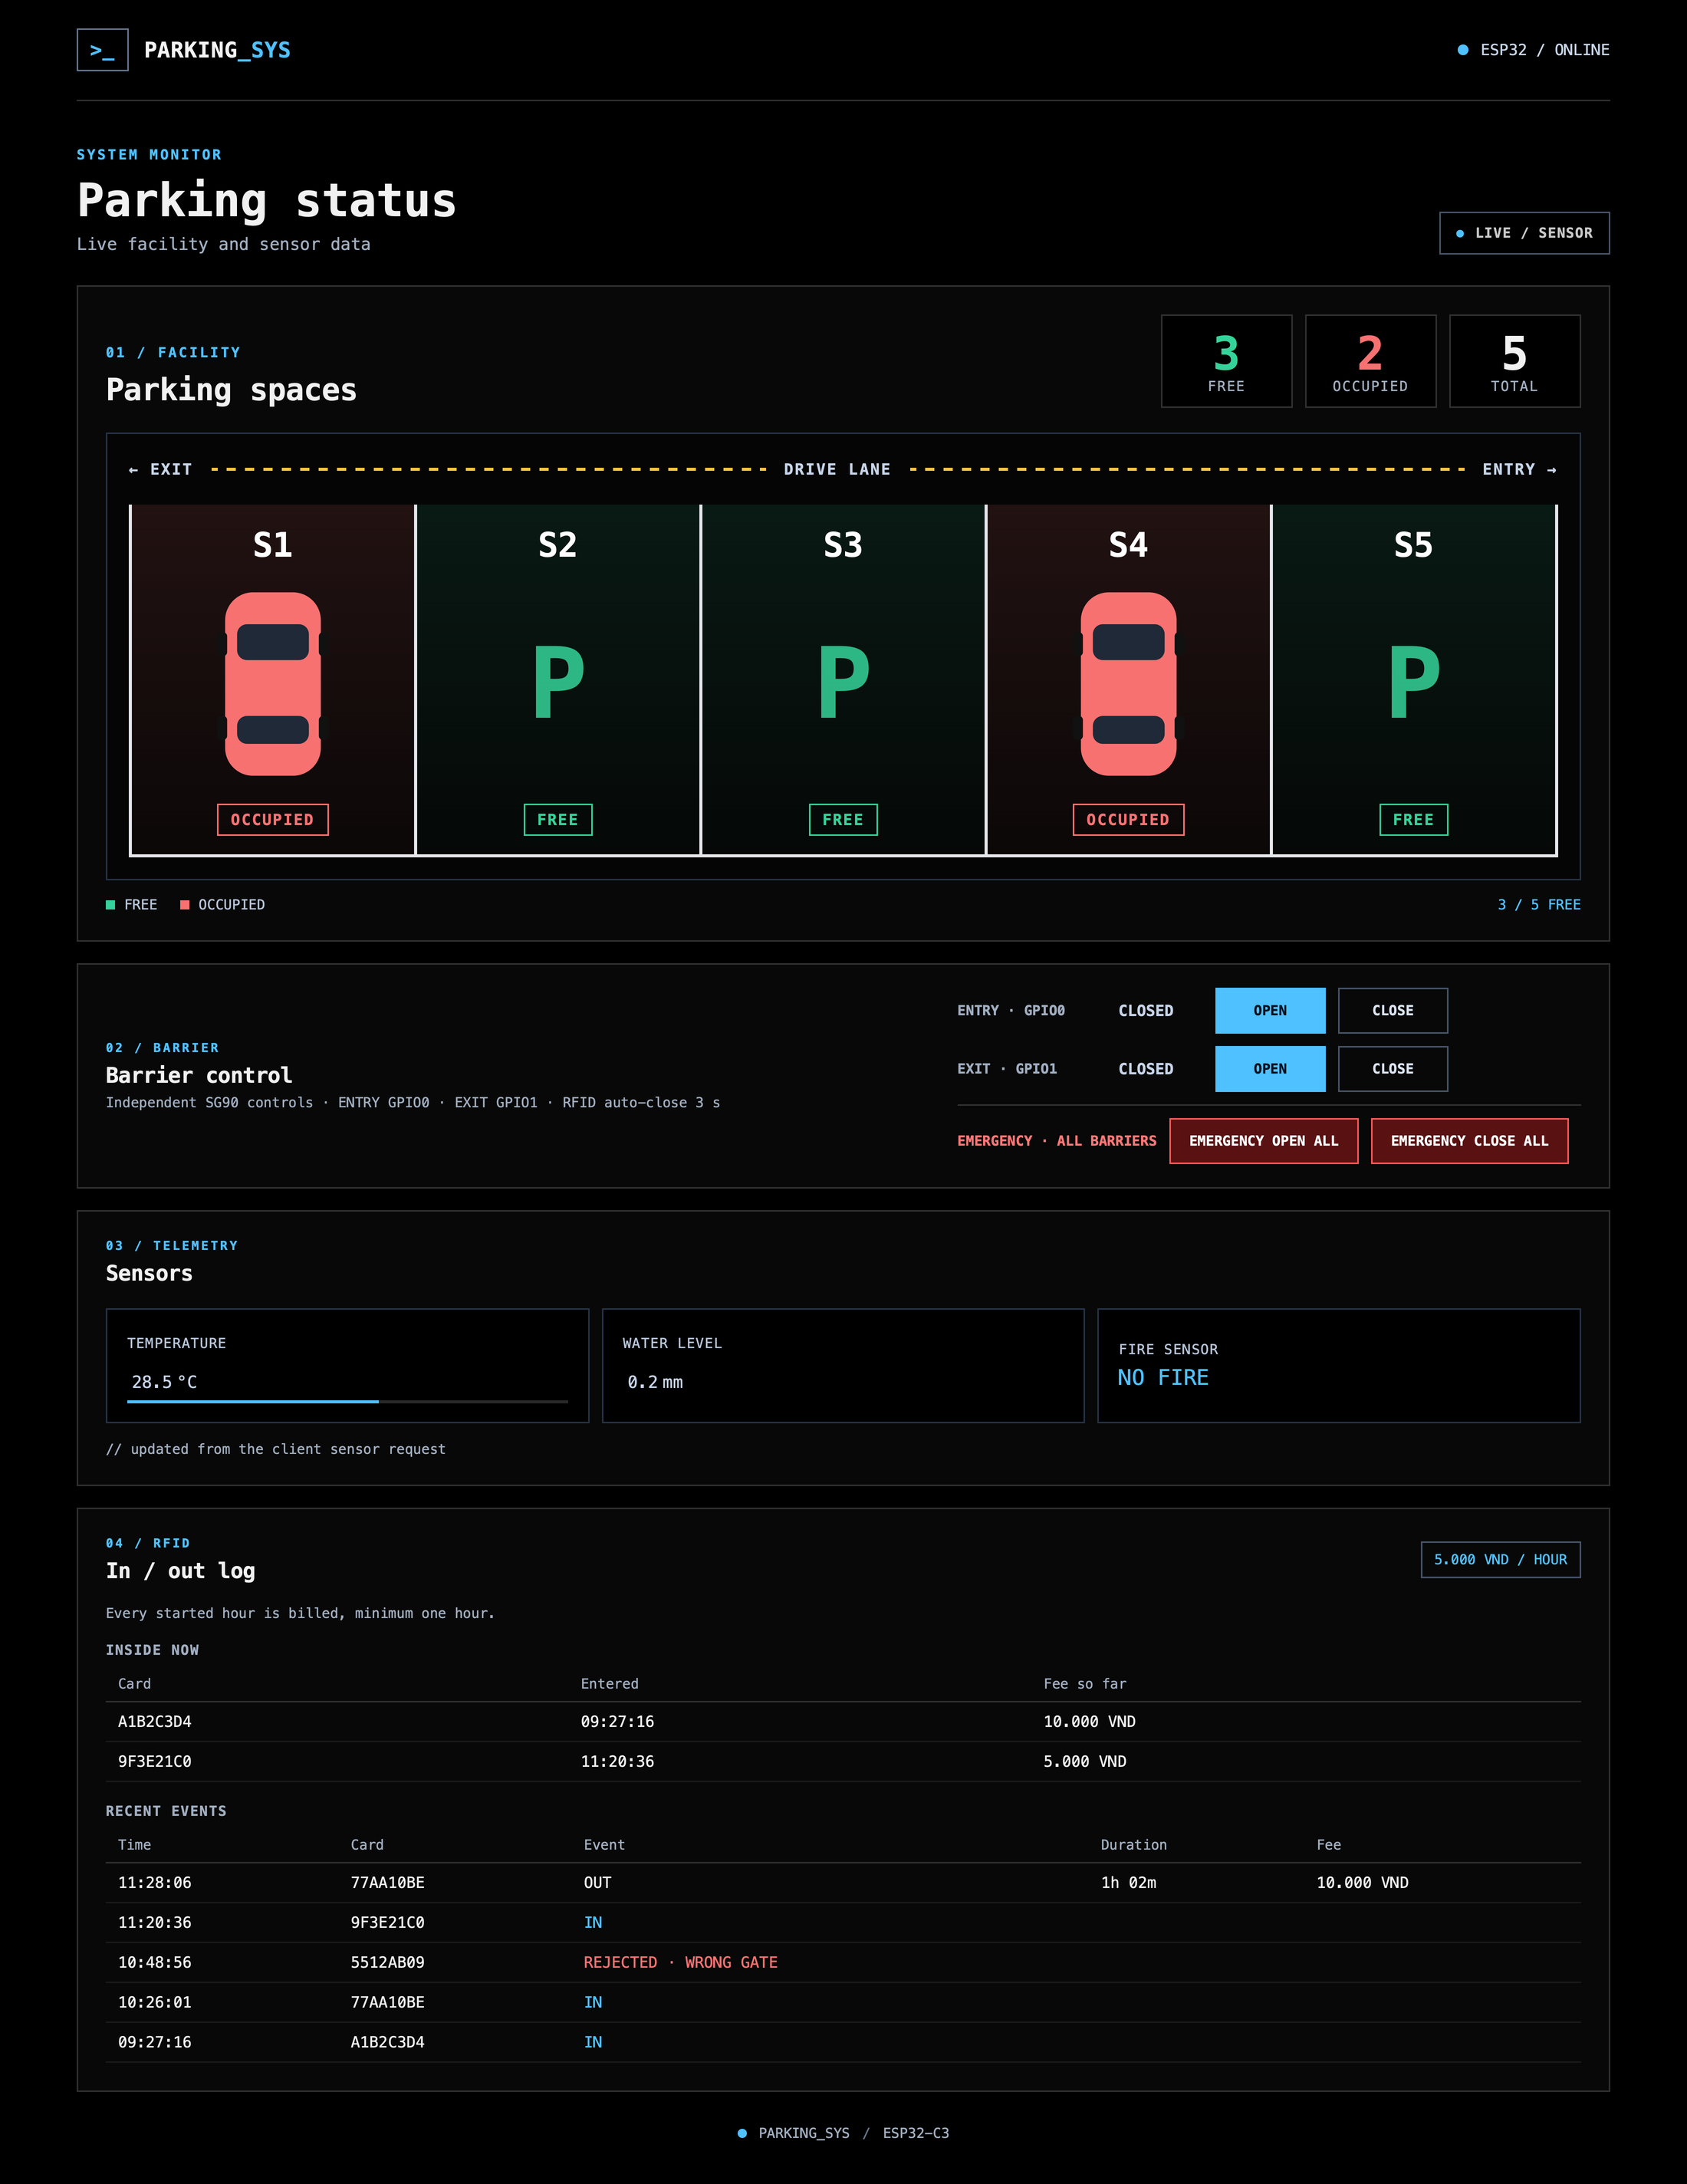
\includegraphics[width=0.86\linewidth]{dashboard.png}
\caption{Trang web giám sát tại \code{http://parking.local} (dữ liệu mẫu)}\label{fig:dashboard}
\end{figure}

\subsection{Các màn hình TFT}
\begin{figure}[H]
\centering
\setlength{\tabcolsep}{3pt}
\begin{tabular}{ccc}
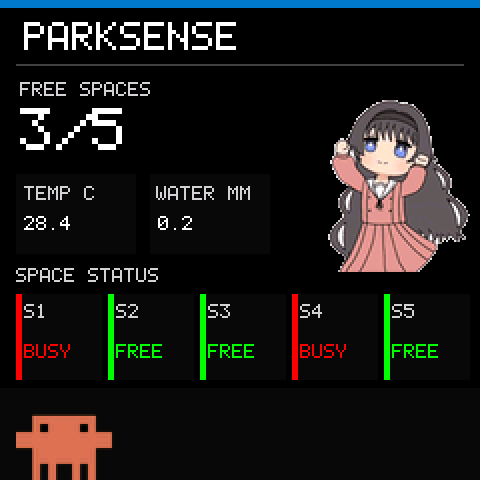
\includegraphics[width=0.3\linewidth]{photos/tft_main.png} &
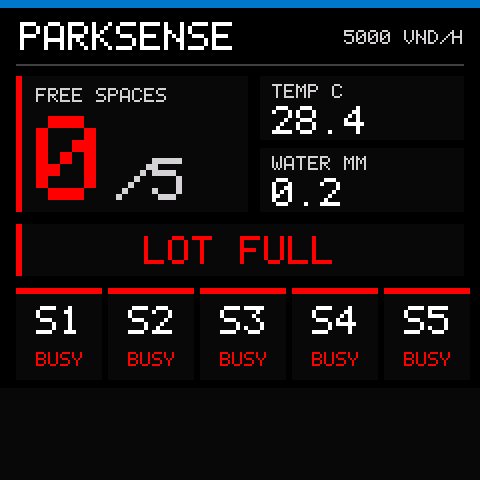
\includegraphics[width=0.3\linewidth]{photos/tft_full.png} &
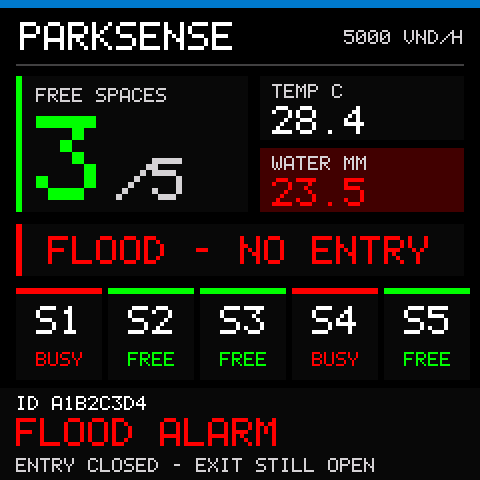
\includegraphics[width=0.3\linewidth]{photos/tft_flood.png} \\
\footnotesize (a) Bình thường & \footnotesize (b) Bãi đầy & \footnotesize (c) Ngập, quẹt vào bị từ chối \\[4pt]
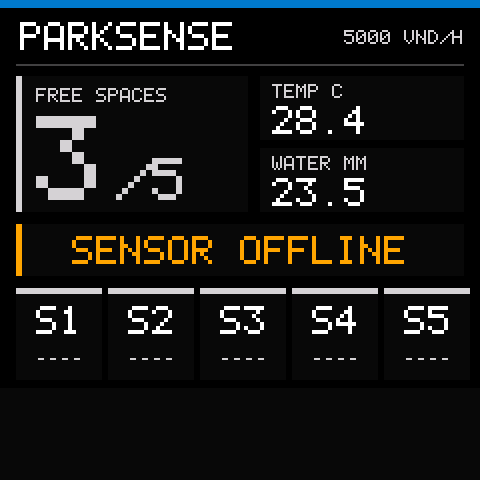
\includegraphics[width=0.3\linewidth]{photos/tft_offline.png} &
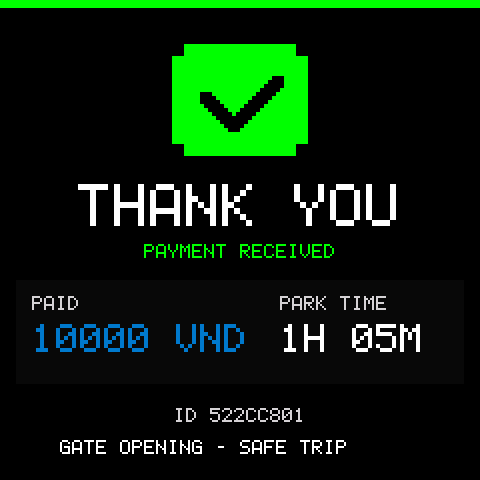
\includegraphics[width=0.3\linewidth]{photos/tft_thanks.png} &
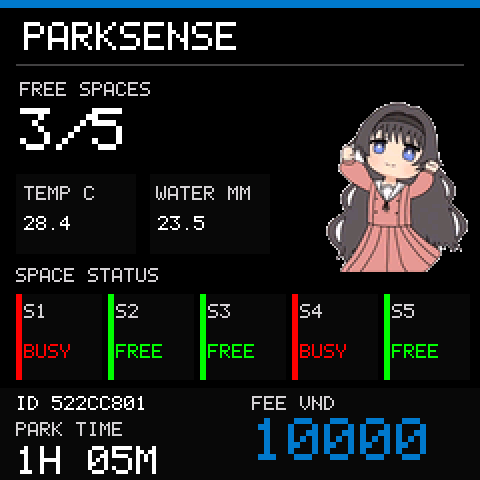
\includegraphics[width=0.3\linewidth]{photos/tft_receipt.png} \\
\footnotesize (d) Cảm biến mất kết nối & \footnotesize (e) Cảm ơn sau khi trả tiền & \footnotesize (f) Hóa đơn ở chân màn hình \\
\end{tabular}
\caption{Các màn hình TFT $240\times240$, kết xuất từ chính mã \file{lcd\_display.c} biên dịch trên máy tính}\label{fig:tft}
\end{figure}
Trên màn hình bình thường: hàng trên là số chỗ trống, hai ô nhiệt độ và mực nước (ô nước chuyển
đỏ khi ngập), ảnh động $96\times96$ ở góc phải; nhãn \code{FLOOD-NO ENTRY} hoặc \code{SENSOR OFFLINE}
hiện ở góc trên; hàng giữa là 5 ô S1–S5 với vạch xanh (trống)/đỏ (có xe); vùng chân dùng cho ảnh
động nhỏ, hóa đơn hoặc thông báo. Khi một lượt trả tiền hoàn tất (SePay hoặc
\emph{Confirm paid}), màn hình \code{THANK YOU} hiện 5\,s trong lúc thanh chắn mở, sau đó hóa đơn
vẫn ở chân màn hình thêm khoảng một phút.

\begin{figure}[H]
\centering
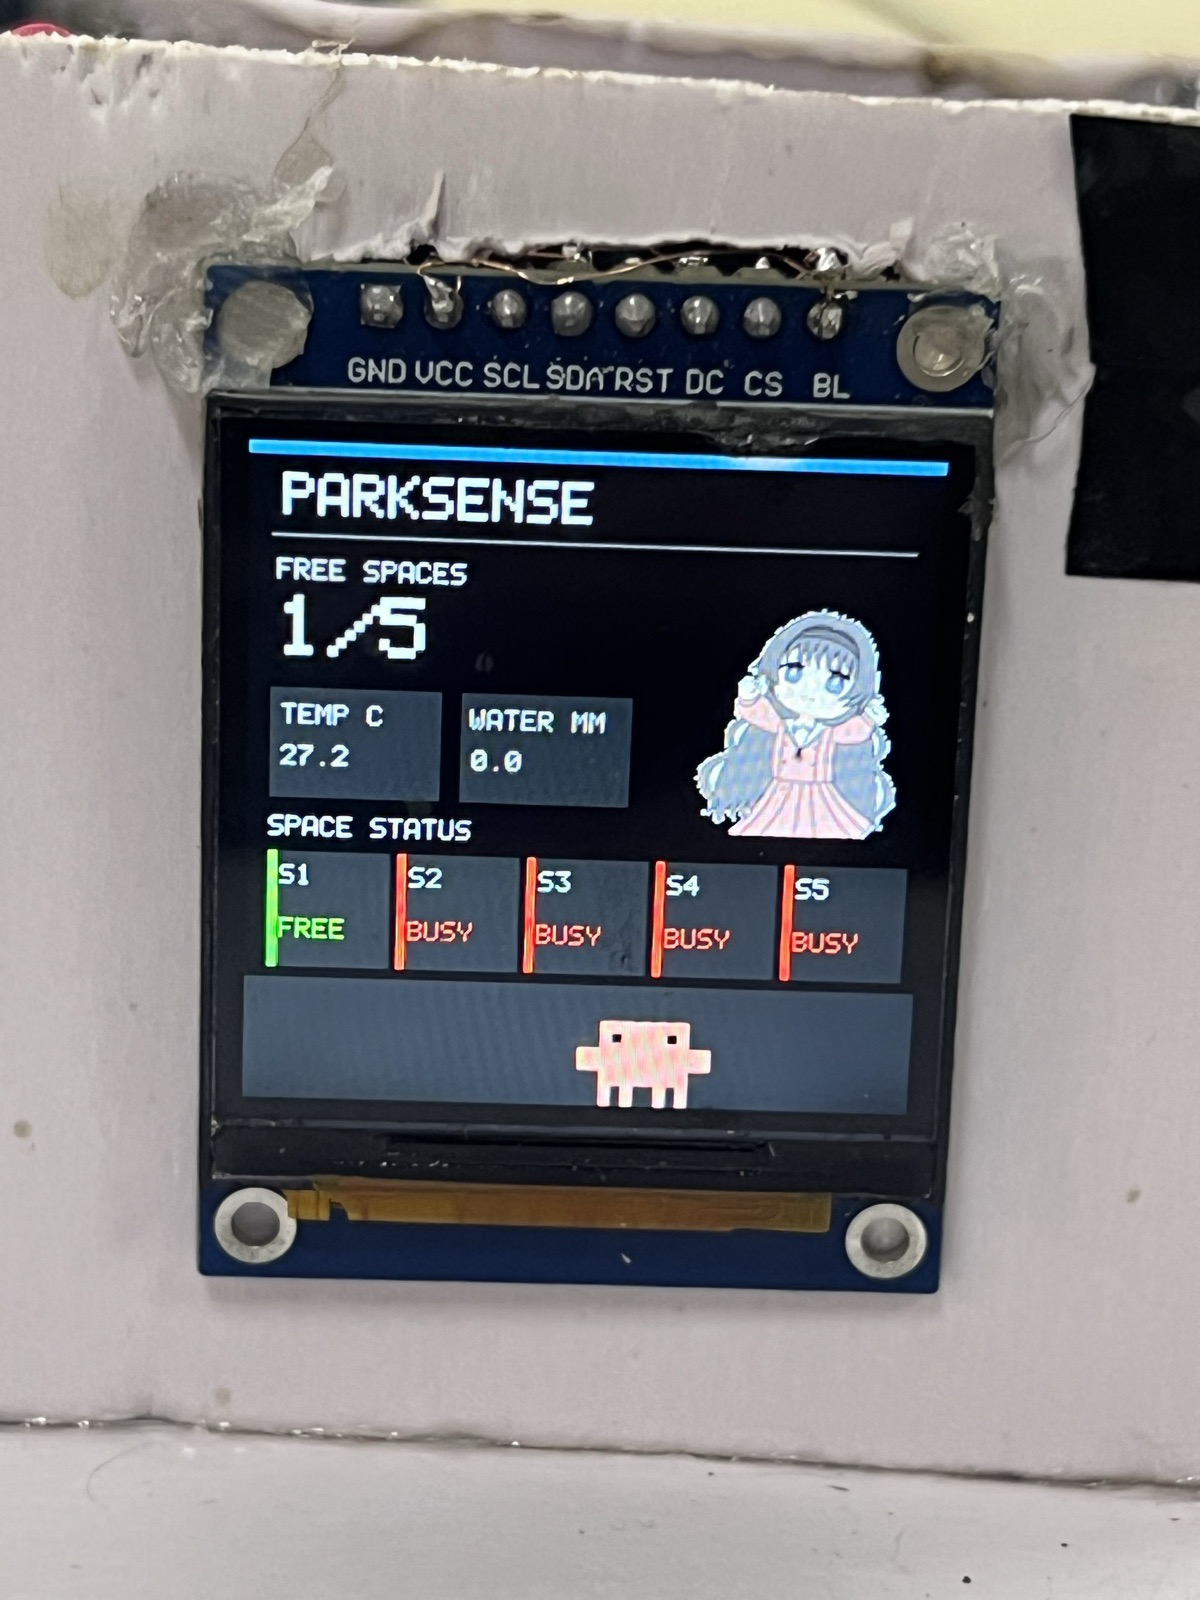
\includegraphics[width=0.42\linewidth]{photos/tft_live.jpg}
\caption{Màn hình TFT thật trên mô hình khi 4 ô có xe: \code{FREE SPACES 1/5}, S1 trống (xanh), S2–S5 có xe (đỏ), nhiệt độ 27,2\,°C, mực nước 0,0\,mm}\label{fig:tft-live}
\end{figure}

\subsection{Kịch bản demo}
\begin{enumerate}
\item Bật máy chủ, RFID Client, Sensor Client (thứ tự bất kỳ); điện thoại ở cùng mạng Wi-Fi chung mở \code{http://parking.local}.
\item Đặt xe mô hình vào ô S2: ô S2 trên TFT chuyển đỏ ngay, trên web hiện hình xe trong $\le$ 1\,s.
\item Quẹt thẻ ở cổng vào: thanh chắn vào mở rồi tự đóng sau 3\,s; web có dòng \code{IN}.
\item Quẹt lại thẻ đó ở cổng vào: màn hình báo \code{WRONG GATE – ALREADY INSIDE - USE EXIT GATE}.
\item Quẹt thẻ ở cổng ra: TFT hiện mã VietQR; quét bằng ứng dụng ngân hàng và chuyển khoản; vài giây sau hóa đơn hiện trên TFT, thanh chắn ra mở; web có dòng \code{OUT} kèm phí.
\item Đưa bật lửa gần cảm biến lửa: còi kêu, màn hình DANGER, hai thanh chắn mở và không đóng được từ web.
\item Tắt lửa: còi tắt, thanh chắn đóng, màn hình trở lại bình thường.
\end{enumerate}

